% A LaTeX (non-official) template for ISAE projects reports
% Copyright (C) 2014 Damien Roque
% Version: 0.2
% Author: Damien Roque <damien.roque_AT_isae.fr>

\documentclass[a4paper,12pt]{book}
\usepackage[utf8]{inputenc}
\usepackage[T1]{fontenc}
\usepackage[frenchb]{babel} % If you write in French
\usepackage{a4wide}
\usepackage{graphicx}
\graphicspath{{images/}}
\usepackage{subfig}
\usepackage{tikz}
\usetikzlibrary{shapes,arrows}
\usepackage{pgfplots}
\pgfplotsset{compat=newest}
\pgfplotsset{plot coordinates/math parser=false}
\newlength\figureheight
\newlength\figurewidth
\pgfkeys{/pgf/number format/.cd,
set decimal separator={,\!},
1000 sep={\,},
}
\usepackage{ifthen}
\usepackage{ifpdf}
\ifpdf
\usepackage[pdftex]{hyperref}
\else
\usepackage{hyperref}
\fi
\usepackage{color}
\hypersetup{%
colorlinks=true,
linkcolor=black,
citecolor=black,
urlcolor=black}

\renewcommand{\baselinestretch}{1.05}
\usepackage{fancyhdr}
\pagestyle{fancy}
\fancyfoot{}
\fancyhead[LE,RO]{\bfseries\thepage}
\fancyhead[RE]{\bfseries\nouppercase{\leftmark}}
\fancyhead[LO]{\bfseries\nouppercase{\rightmark}}
\setlength{\headheight}{15pt}

\let\headruleORIG\headrule
\renewcommand{\headrule}{\color{black} \headruleORIG}
\renewcommand{\headrulewidth}{1.0pt}
\usepackage{colortbl}
\arrayrulecolor{black}

\fancypagestyle{plain}{
  \fancyhead{}
  \fancyfoot[C]{\thepage}
  \renewcommand{\headrulewidth}{0pt}
}

\makeatletter
\def\@textbottom{\vskip \z@ \@plus 1pt}
\let\@texttop\relax
\makeatother

\makeatletter
\def\cleardoublepage{\clearpage\if@twoside \ifodd\c@page\else%
  \hbox{}%
  \thispagestyle{empty}%
  \newpage%
  \if@twocolumn\hbox{}\newpage\fi\fi\fi}
\makeatother

\usepackage{amsthm}
\usepackage{amssymb,amsmath,bbm}
\usepackage{array}
\usepackage{bm}
\usepackage{multirow}
\usepackage[footnote]{acronym}

\newcommand*{\SET}[1]  {\ensuremath{\mathbf{#1}}}
\newcommand*{\VEC}[1]  {\ensuremath{\boldsymbol{#1}}}
\newcommand*{\FAM}[1]  {\ensuremath{\boldsymbol{#1}}}
\newcommand*{\MAT}[1]  {\ensuremath{\boldsymbol{#1}}}
\newcommand*{\OP}[1]  {\ensuremath{\mathrm{#1}}}
\newcommand*{\NORM}[1]  {\ensuremath{\left\|#1\right\|}}
\newcommand*{\DPR}[2]  {\ensuremath{\left \langle #1,#2 \right \rangle}}
\newcommand*{\calbf}[1]  {\ensuremath{\boldsymbol{\mathcal{#1}}}}
\newcommand*{\shift}[1]  {\ensuremath{\boldsymbol{#1}}}

\newcommand{\eqdef}{\stackrel{\mathrm{def}}{=}}
\newcommand{\argmax}{\operatornamewithlimits{argmax}}
\newcommand{\argmin}{\operatornamewithlimits{argmin}}
\newcommand{\ud}{\, \mathrm{d}}
\newcommand{\vect}{\text{Vect}}
\newcommand{\sinc}{\ensuremath{\mathrm{sinc}}}
\newcommand{\esp}{\ensuremath{\mathbb{E}}}
\newcommand{\hilbert}{\ensuremath{\mathcal{H}}}
\newcommand{\fourier}{\ensuremath{\mathcal{F}}}
\newcommand{\sgn}{\text{sgn}}
\newcommand{\intTT}{\int_{-T}^{T}}
\newcommand{\intT}{\int_{-\frac{T}{2}}^{\frac{T}{2}}}
\newcommand{\intinf}{\int_{-\infty}^{+\infty}}
\newcommand{\Sh}{\ensuremath{\boldsymbol{S}}}
\newcommand{\C}{\SET{C}}
\newcommand{\R}{\SET{R}}
\newcommand{\Z}{\SET{Z}}
\newcommand{\N}{\SET{N}}
\newcommand{\K}{\SET{K}}
\newcommand{\reel}{\mathcal{R}}
\newcommand{\imag}{\mathcal{I}}
\newcommand{\cmnr}{c_{m,n}^\reel}
\newcommand{\cmni}{c_{m,n}^\imag}
\newcommand{\cnr}{c_{n}^\reel}
\newcommand{\cni}{c_{n}^\imag}
\newcommand{\tproto}{g}
\newcommand{\rproto}{\check{g}}
\newcommand{\LR}{\mathcal{L}_2(\SET{R})}
\newcommand{\LZ}{\ell_2(\SET{Z})}
\newcommand{\LZI}[1]{\ell_2(\SET{#1})}
\newcommand{\LZZ}{\ell_2(\SET{Z}^2)}
\newcommand{\diag}{\operatorname{diag}}
\newcommand{\noise}{z}
\newcommand{\Noise}{Z}
\newcommand{\filtnoise}{\zeta}
\newcommand{\tp}{g}
\newcommand{\rp}{\check{g}}
\newcommand{\TP}{G}
\newcommand{\RP}{\check{G}}
\newcommand{\dmin}{d_{\mathrm{min}}}
\newcommand{\Dmin}{D_{\mathrm{min}}}
\newcommand{\Image}{\ensuremath{\text{Im}}}
\newcommand{\Span}{\ensuremath{\text{Span}}}

\newtheoremstyle{break}
  {11pt}{11pt}%
  {\itshape}{}%
  {\bfseries}{}%
  {\newline}{}%
\theoremstyle{break}

%\theoremstyle{definition}
\newtheorem{definition}{Définition}[chapter]

%\theoremstyle{definition}
\newtheorem{theoreme}{Théorème}[chapter]

%\theoremstyle{remark}
\newtheorem{remarque}{Remarque}[chapter]

%\theoremstyle{plain}
\newtheorem{propriete}{Propriété}[chapter]
\newtheorem{exemple}{Exemple}[chapter]

\parskip=5pt
%\sloppy

\begin{document}

%%%%%%%%%%%%%%%%%%
%%% First page %%%
%%%%%%%%%%%%%%%%%%

\begin{titlepage}
\begin{center}


\includegraphics[width=0.6\textwidth]{uvsq-logo-rvb-def}\\[1cm]

{\large Sécurité des Contenus, des Réseaux, des Télécommunications et des Systèmes}\\[0.5cm]

{\large Rapport de stage}\\[0.5cm]

% Title
\rule{\linewidth}{0.5mm} \\[0.4cm]
{ \huge \bfseries Amélioration des process d'audit et de collecte des indicateurs de sécurité des sites web publics du groupe Schneider-Electric\\[0.4cm] }
Société d'accueil : Schneider-Electric Grenoble
\rule{\linewidth}{0.5mm} \\[1.5cm]


% Author and supervisor
\noindent
\begin{minipage}{0.4\textwidth}
  \begin{flushleft} \large
    \emph{Auteurs :}\\
    M. Pazisnéwendé Aubain  \textsc{Tapsoba}\\

  \end{flushleft}
\end{minipage}%
\begin{minipage}{0.4\textwidth}
  \begin{flushright} \large
    \emph{Maître de stage :} \\
    Mme. Siham \textsc{Benhamidouche}\\
  
  \end{flushright}
\end{minipage}

\vfill

% Bottom of the page
{\large Période du 03 Avril au 03 Octobre \\ Année académique 2017-2018}

\end{center}
\end{titlepage}

%%%%%%%%%%%%%%%%%%%%%%%%%%%%%
%%% Non-significant pages %%%
%%%%%%%%%%%%%%%%%%%%%%%%%%%%%

\frontmatter

\chapter*{Remerciements}
Mes remerciements 

\clearpage
\tableofcontents

\clearpage
\listoffigures

\clearpage
\chapter*{Liste des sigles et acronymes}
\begin{acronym}[CP-OFDMX] % Give the longest acronym here
\acro{DEVOPS}{\emph{Developpement and Operations}}
\acro{POC}{\emph{Proof Of Concept}}
\end{acronym}

%%%%%%%%%%%%%%%%%%%%%%%%%%%%%%%%%%%%%%%%%%%%
%%% Content of the report and references %%%
%%%%%%%%%%%%%%%%%%%%%%%%%%%%%%%%%%%%%%%%%%%%

\mainmatter
\pagestyle{fancy}

\cleardoublepage

\chapter*{Introduction générale}
\vspace*{-1.1cm}
Les thématiques de la sécurité informatique s’invitent depuis plusieurs années aux sujets des préoccupations majeures des organisations et des entreprises. 
De son ampleur, certaines entreprises à juste titre lui confèrent le titre de domaine critique et sensible. 
Selon les conclusions du rapport de Verizon parut en 2017, 77\% des organisations dans le monde ont été touché par des cyber-attaques au cours de l’année 2017. \newline
Ces attaques ont des impacts forts sur l’économie et sur la réputation des victimes. Dans ce contexte, il apparaît clairement la nécessité pour les entreprises d’améliorer la sécurité de leur système d’information.
Ce processus d’amélioration passe par la formation de la ressource humaine d’une part et par des réalisations techniques sûres d’autre part. \newline
En particulier, techniquement l’amélioration de la sécurité d’une entreprise se produit en amont de la phase de production par l’amélioration de la sécurité et en aval par le mise en place de techniques de défense, de détection et de gestion des incidents de sécurité de ce produit.\newline
La maîtrise de ces techniques est la problématique actuelle des acteurs de la cybersécurité et de toutes les entreprises émettant des produits électroniques et informatiques. 
Ainsi afin de s’assurer la maîtrise de ces processus, Schneider-Electric s'est doté de plusieurs pôles dédiés au monitoring, à la gestion des incidents et enfin charger de les prévenir prévention. 

De ces besoins exprimés, nous avons été accueillis au sein du groupe SE pour un stage de 6 mois durant lequel, nous avons travaillé sur l’amélioration des indicateurs de sécurité de notre société d'accueil d'une part et sur la mise en place d'un POC de certification continue d'autre part. 
\newline En effet notre stage au sein du groupe SE s’est construit autour du sujet « Amélioration des indicateurs de sécurité des sites web publics du groupe SE », nous avons donc travailler sur l’intégration des indicateurs de sécurité en amont de la phase de production et en avale sur le monitoring des indicateurs de sécurité. 
\newline Le présent document, synthèse de nos activités durant le stage s’articule sur 3 parties. 
Dans la première partie, nous procéderons à la présentation de notre entreprise d’accueil, ainsi que les objectifs généraux de notre stage. 
\newline
Dans la deuxième partie, nous présenterons d'abord le métier que nous avons appris, ensuite nous aborderons des solutions que nous avons proposé. 
\newline
Dans la troisième partie du rapport, il sera question de nos réalisations dans la mise en oeuvre d'un \ac{POC} pour la mise en oeuvre des concepts de certification continue dans le cadre d'un projet \ac{DEVOPS}.

\part{Etudes préalables }
\chapter{La société d'accueil}
\section*{Introduction}
\section{Présentation}
Schneider-Electric est une multinationale Française spécialisée dans les automatismes et dans la gestion de l’énergie.\newline 
Elle intervient particulièrement dans la conception, la gestion, la réalisation des solutions techniques innovantes et dans la proposition de services autour des projets électriques. \newline
Sa mission principale est de mettre à la disposition de ses clients des produits à haute valeur ajoutée afin de les accompagner dans leur stratégie de gestion de l’énergie.\newline


Fondée au 19è siècle par les frères Schneider, la société a en 180 années su remporter de nombreux défis et devenir un acteur majeur dans tous les niveaux des offres électriques. De nos jours, elle se positionne comme une entreprise innovante, et engagée dans la transition énergétique, dans le développement des outils intelligents et dans la formation des jeunes.


Sur le territoire Français la société compte plus de 100 sites, plus de 150 milles collaborateurs et produit un chiffre d'affaire annuel supérieur à 1,7 milliard d'euros depuis 2013.\newline
De son leadership dans son domaine, elle est la cible de plusieurs attaques informatiques. Ces attaques visent pour l’essentiel la base de connaissance du groupe, et pour d’autres l'objectif est de ternir la réputation de la société auprès de ses clients.
Aussi il importe de mettre aux devants au vu de l'importance du groupe les potentiels espionnages dont il pourrait être l'objet.


\section{Organisation interne}
Schneider-Electric est une société européenne à conseil d’administration. Elle applique le code de gouvernance des entreprises et des sociétés cotées. 
Selon les recommandations de cette gouvernance, elle dispose d’un conseil d’administration en charge de déterminer les orientations de l’activité de la Société et veille à leur mise en œuvre. 
\newline 
A la suite du conseil d'administration suivent respectivement la direction du groupe et le comité exécutif. La direction du groupe représente la société dans ses rapports avec les tiers. Elle est investi des pouvoirs les plus étendus pour agir en toutes circonstances au nom de la société. 
\newline
Le comité exécutif, quant à lui est en charge de supporter et de mettre en opération les décisions du conseil d'administration. 

\section{Aperçu sur l'architecture Informatique}
De part son choix de développement et de sa répartition géographique, la société dispose d’une architecture informatique distribuée et hétérogène.
De partout dans le monde, elle dispose de plusieurs datacenters sur lesquels sont déployés les applications dites sensibles.
\newline
A côté de ces applications dites sensibles, il en existe celles à faible valeur ajoutée qui se retrouvent souvent chez des fournisseurs tiers.

Aussi certaines acquisitions du groupe gère elle-même leur système d’information qui n’ont souvent aucune connexion avec celui du groupe. Cette situation singulière intervient particulièrement lorsque l'intégration du Système d'information de la société rachetée va entraîner une régression de sécurité chez l'une des deux sociétés. 

\section{Quelques attaques informatiques sur le groupe}
Faisant un stage en sécurité informatique au sein du groupe, il nous a paru nécessaire pour nous de recenser les attaques et les vulnérabilités marquantes auxquelles le groupe a déjà été exposé.  
\subsection{Exploitation d'une vulnérabilités sur le triconnex}
Cette attaque fut signalée par la \ac{FBI}. Elle date de l’année 2015. Elle a touché une filiale du groupe spécialisée dans le développement des logiciels de supervision de pipeline. Cette attaque a eu pour conséquence l’ex-filtration de données massives. 
\newline
Par ailleurs, elle a eu des conséquences économiques, et a également eu des impacts négatifs sur la réputation du groupe.  

\subsection{Vulnérabilités sur le SCADA}
De facon chronologique, il eût d'abord celles de Septembre 2012. en effet, durant cette periode, la filiale TELVENT de Schneider-Electric, spécialisée dans les systèmes de contrôle industriels énergétiques, a été victime d’une attaque réseau. Des attaquants d’origine chinoise ont réussi à contourner les pares-feux de TELVENT, et, après avoir investi des pans entiers de son réseau, y ont installé des logiciels malicieux afin de dérober des données sur un SCADA.
\newline
Ensuite, en 2018, de multiples vulnérabilités ont été découvertes dans SCADA les produits Schneider-Electric le 12 février 2018 par le CERT de la France. Elles permettent à un attaquant de provoquer une exécution de code arbitraire à distance, une atteinte à l'intégrité des données et une atteinte à la confidentialité des données.

\section*{Conclusion}
Dans ce chapitre, nous avons eu une appercu générale sur les domaines d'intervention du groupe d'une part et 

\chapter{Contexte du stage}
\section*{Introduction}
\section{Le stage}
Le Master II SéCRéTS est une formation de l’université Paris-Saclay, un consortium de trois universités, de neuf grandes écoles et de sept organismes de recherches. \newline
Cette formation a pour but d’apporter aux étudiants une compréhension fine des défis liés d’une part, à la conception de systèmes sûrs et d’autres part à fournir des bases théoriques, pratiques et solides sur les concepts et les enjeux de la cybersécurité. \newline
La validation de ce Master est jalonnée par un stage de six mois minimums et obligatoire à réaliser auprès des professionnels de la sécurité informatique. 
En particulier, ce stage a pour objectifs : 
\begin{itemize}
    \item[•]	de permettre à l’étudiant d’apprendre de son futur métier ;
    \item [•]	de permettre à l’étudiant d’avoir un encadrement avant son immersion totale dans le monde professionnel ;
    \item [•]	de profiter des retours des entreprises afin de mieux adapter la formation. 
\end{itemize}


Dans le cadre de ma formation, j’ai été reçu en stage de 6 mois au sein de l’équipe DCX Security de la société Schneider-Electric. Dans cette équipe nous avons pu travailler principalement sur le sujet \textbf{« Amélioration des process d'audit et de collecte des indicateurs de sécurité des sites web publics du groupe Schneider-Electric »}. 

Ce stage devrait être l’occasion pour nous d’approfondir nos connaissances sur les sujets de la sécurité des applications web en particulier, dans la sécurité opérationnelle, dans le monitoring et dans la réponse aux incidents des applications web en général. 

\section{Equipe d’accueil}
\subsection{Présentation}
Nous avons été accueilli au sein de l’équipe DCX Security. Cette équipe est managée par Siham Benhamidouche, Digital Risk Leader, et compte en tout 3 collaborateurs.


Elle est entre autres en charge de la sécurité des applications web, de celle du DNS et de celle des applications sensibles. 
\newline Particulièrement les missions principales de l’équipe sont de veiller à la sécurité des applications web et mobiles publiques du groupe, cela en passant par la surveillance des indicateurs de sécurité d’un site web.


Pour l’atteinte de ces objectifs, elle passe par plusieurs missions : de la rédaction de supports, à l’amélioration des notes, en passant par la gestion des incidents et l’amélioration des process, nous avons pu apporter notre contribution à la vie de l’équipe et à l’atteinte des objectifs assignés à l’équipe. 


\subsection{Objectifs de l'équipe}
A notre arrivée au sein de l'équipe nous avons d’abord voulu comprendre ses métiers. Passée cette étape, nous avons voulu comprendre les difficultés auxquelles faisaient face l’équipe. De cette étape, nous avons pu rassembler les missions suivantes : 
\begin{itemize}
    \item[•] améliorer les notes de sécurité du groupe Schneider-Electric ; 
    \item[•] rédiger des politiques et standards de sécurité pour les sites web ;
    \item[•] rédiger des guides de configurations sûres ;
    \item[•] sensibiliser sur la sécurité des applications web ; 
    \item[•] être le réfèrent technique pour les vulnérabilités web et mobiles; 
    \item[•] réagir aux incidents de sécurité relatif aux technologies inhérents à celles du web.
\end{itemize}
Dans la mise en oeuvre de ses missions, l'équipe fait face à plusieurs difficultés. Parmi ces dernières, nous avons pu observer :
\begin{itemize}
   \item[•] identification des propriétaires des systèmes présentant des incidents ;
   \item[•] distribution du système d’information du groupe rend difficile les traitements en masse ; 
   \item[•] anticipation difficile dans l’identification des systèmes présentant des problèmes de sécurité ;
   \item[•] mise à jour rapide des politiques de sécurité.
\end{itemize}

\section{Objectifs du stage}
Les objectifs de notre stage ont été à la fois de participer à l’atteinte des objectifs de l’équipe d’une part, et de proposer des solutions aux difficultés exprimées plus haut d’autre part. En accord avec le sujet du stage « Amélioration des indicateurs de sécurité des sites web publics du groupe SE » nous avons travaillé sur l’amélioration des notes de sécurité du groupe Schneider-Electric et sur la certification des applications en amont. 
Ces travaux devraient permettre à l’équipe de façon générale : 
\begin{itemize}
    \item[•] améliorer les scores de sécurité du groupe ;
    \item[•] disposer de plus d’outils de checks de la sécurité des applications web ;
    \item[•] intégrer des tests de sécurité durant le processus de certification des applications ;
\end{itemize}

\section{Résultats attendus}
Le résultat général attendu à l'issue de ce stage était l'amélioration des scores de sécurité de Schneider-Electric délivrés par les agences de notation cyber.
Ainsi, nous étions libre de proposer toute solution qui permettrait d'attendre ce résultat. 
De part l'orientation de notre formation, nous avons pris position sur les questions techniques. 

Ainsi comme résultats particuliers de notre stage, nous devrions proposer des POC  qui aiderait l'équipe à devenir plus efficace d'une part et d'autre part des POC qui permettrait de produire des applications plus sures et plus conformes aux politiques de sécurité du groupe.

\section*{Conclusion}

\part{Amélioration des notes de sécurité du groupe}

\chapter{Etude de l'existant}
\section*{Introduction}
L’objet de chapitre est de présenter le système de surveillance de sécurité adopté par le groupe Schneider-Electric. Aussi il aura pour objet de présenter la problématique et les objectifs assignés a cette partie du stage.  

\section{Surveillance de sécurité}
Au vu de son modèle de développement, le groupe a opté pour un système de surveillance géré par des entreprises externes. Ces entreprises sont des agences de notation spécialisée dans la cybersécurité. Elles scannent de façon régulière le réseau Internet et établissent sur la base des remontées des notes qu’elles assignent à ses clients scannés. 


Ce choix se justifie amplement par le besoin pour la société de pouvoir évaluer rapidement et simplement son niveau de cybersécurité. Il s’agit là, d’une attente de la direction générale, toujours dans la volonté de s'auto-évaluer par rapport aux autres entreprises du même secteur, voir à leurs concurrents. 

\section{Les agences de notation cyber}
\subsection{Présentation}
\subsection{Mode opératoire}
Les plate-formes de notation spécialisées en cybersécurité collectent, grâce à différentes sondes et connecteurs sur le réseaux internet, trois types de données :
\begin{itemize}
    \item des données sur les activités malicieuses ; 
    \item des «data feed» fournis par les «vendors», éditeurs de logiciels et de systèmes de sécurité et acteurs spécialisés en «threat intelligence» ; 
    \item des «data feed» propriétaires constitués à partir des analyses de vulnérabilités externes régulières sur les réseaux des entreprises évaluées et des capteurs positionnés en divers endroits du réseau internet.
\end{itemize}
Ces données sont ensuite agrégées et permettent, grâce à des algorithmes non révélés, d’établir des notes par grands indicateurs, puis une note globale pour chaque société. 
\subsection{Techniques de collectes}
Les techniques de collecte sont fortement dépendante de l'agence de notation et du type de données à collecter. Nous avons pu recouvrir trois techniques de collectes utilisées par la majorité des agences de notation cyber. Ainsi nous avons eu :

Les techniques utilisées pour la détection des systèmes éventuellement compromis sont celles du sinkhole et ou du honeypot. Dans cette technique, dans un premier temps, il s’agit de diriger tous les flux entrants et sortants de la machine suspecte tout en simulant un comportement normal vers un système saint et contrôlé. Puis dans une seconde mesure dans le système contrôlé, scinder les flux normaux des flux malicieux en vue d'en faire une analyse afin de déterminer le type d’infection dont est l'objet la machine.


Celles utilisées pour la détection des spams indésirables sont celles dites de spam trapping. Il s'agit d'une adresse mail qui n’est utilisé que par personne, ainsi tous les mails à destination de cette adresse sont potentiellement des spams. 

Enfin nous avons les techniques de scans passifs, qui sont fait directement sur internet afin de déterminer les services et les potentielles vulnérabilités des services exposés.

\subsection{Les indicateurs}
Au même titre que les techniques de collecte, les indicateurs  sont fortement dépendants des agences de notation. de l'ordre du général, nous avons constater que ces indicateurs sont regroupés en catégorie. Ces catégories sont quasi similaires dans les deux agences de notation en charge de noter le groupe la sécurité des applications et sites web du groupe Schneider-Electric.
Ainsi avons-nous les catégories Spam propagation, botnet infection, malware servers, potentially exploited, et dilligence. 
De façon détaillée, 
\begin{description}
    \item[Spam propagation :]cet incident est remonté quand au sein de l’entreprise, il existe une application malicieuse qui envoie des mails commerciaux indésirables. Il est remonté par les techniques de spam trap. Il a pour conséquence de nuire à la réputation de l’entreprise.  
    \item[Botnet infection :] il est reporté quand les agences de notation détecte par l’utilisation d’un sinkhole, des communications de la machine vers un réseau de botnet. Aussi, il remonte cet incident quand il observe des commandes depuis un "command and control server" à destination de la machine scannée. 
    \item[Malware servers :] cette categorie indique qu'un système se livre à des activités malveillantes, telles que l'hébergement de sites de phishing, de fraude ou d'arnaque dans le but de distribuer des logiciels malveillants et des virus. Cet incident peut être annonciateur d’exfiltration de données, d’accès non autorisé et d’abus de ressources, il est principalement par les techniques de sinkhole.  
    \item[Potentially exploited :] cet incident est remonté quand un ordinateur exécute une application potentiellement indésirable qui peut permettre à des logiciels malveillants et plus dangereux de compromettre le système. Il est remonté par les techniques de sinkhole.
    \item [Diligence :]cette catégorie regroupe les bonnes pratiques de défense en profondeur permettant de réduire au maximum la surface d’attaque d’une application/d’une machine et du suivi des mises à jour des applications. Elle regroupe les sous categories suivantes :
    \begin{itemize}
        \item la présence d’un enregistrement SPF;
        \item la presence de l’authentification DKIM;
        \item la validité des certificats SSL;
        \item les configurations SSL;
        \item les ports ouverts ;
        \item les entêtres de sécurité du protocole HTTP dans les application web;
        \item patching Cadence, les protocoles utilisés pour protéger la couche transport;
        \item server Software, les applications utilisées comme serveur ; 
        \item desktop Software, les applications installées en locale; 
        \item mobile Software les applications mobiles ; 
        \item mobile Application Security pour la sécurité de la couche applicative des applications mobiles 
   

    \end{itemize}
    
\end{description}

\subsection{Périodicité et reconnaissance}
Les agences de notation cyber scannent continuellement internet afin de détecter les problèmes de sécurité énoncés plus haut. Elles procèdent essentiellement par trois méthodes afin de déterminer la société propriétaire de l’application scannée : primo, elle détermine le propriétaire de l’adresse IP scannée. Secundo, si cette information n’est pas suffisante pour l’identification, elle essaye de déterminer le \ac{FQDN} de l’application à l’aide d’une résolution DNS inverse. Au cas où elle ne dispose d’aucune information à l’issue des phases précédentes, elle procède à la lecture des |\ac{CNs} et des \ac{SANs} des certificats. 


Ces scans sont effectués de manière continuelle et sont remonté sous forme de tableau. A chaque incident est associé la date du scan, l’adresse IP de la machine scannée et éventuellement le nom DNS de la machine scannée. Aussi, certaines donnent les procédures pour résoudre les incidents.


\section{Analyse du système de surveillance}

\subsection{Avantages}
\subsection{Inconvénients}
\section{Conclusion}



\chapter{POC de traitement des incidents}
\part{Intégration de la sécurité pendant la phase de développement}
\chapter{Le projet de certification continue}
\section{Introduction}
\chapter{Gestion du projet}
\section{Introduction}
Pour mener à bien ce projet, nous avons opté pour une méthode d’organisation efficace, construite autour de la satisfaction du client et de son implication durant tout le cycle du projet. Au regard de ces exigences, notre choix s’est porté sur \ac{SCRUM}.
\newline
Il s'agit d'une méthode agile qui stipule un schéma d’organisation de développement de produits complexes. Il est défini par ses créateurs selon ses termes « un cadre de travail permettant de répondre à des problèmes complexes et changeants tout en livrant de manière productive et créative des produits de la plus grande valeur possible »

\section{les piliers de SCRUM}
\subsection{Transparence}
SCRUM met l'accent sur le fait d'avoir un langage commun entre l'équipe de développement et l’équipe de management. Ce langage commun doit permettre à tout observateur d'obtenir rapidement une bonne compréhension du projet. 

\subsection{Inspection}
À intervalles réguliers, SCRUM propose de faire le point sur les différents artéfacts produits détails, afin de détecter toute variation indésirable. Ces inspections ne doivent pas être faites trop fréquemment : cela nuirait à l'avancement du projet.


\subsection{Adaptation}
Si une dérive est constatée pendant l'inspection, le processus doit alors être adapté. SCRUM fournit des moyens rendant cette adaptation possible. Il s'agit de la réunion de planification de sprint, de la mêlée quotidienne, de la revue de sprint ainsi que de la rétrospective de sprint.

\section{Les rôles dans la gestion du projet}
SCRUM définit trois rôles : le Propriétaire du produit (Product Owner), le SCRUM Master et l’équipe de développement.

\subsection{Le propriétaire du produit}
Le propriétaire du produit (Product Owner) est le représentant des clients et des utilisateurs. Il s'agit d'« une personne et non d'un comité ». Il est seul à diriger l'activité de l'équipe de développement à qui il n'est « pas permis de suivre les instructions d'une autre personne. »
De ce fait, cet acteur se charge de différents rôles et responsabilités. Il explicite les éléments (Items) du carnet de produit (product backlog). Il définit l'ordre dans lequel les fonctionnalités seront développées. Il prend les décisions importantes concernant l'orientation du projet. Il s'assure que le carnet du produit est visible et compris de l'équipe de développement.
Dans notre cas, le propriétaire a été M. Emnuelle Beaugrand, Chargé de la optimisation et de la gouvernance au sein de Schneider-Electric.

\subsection{Le SCRUM master}
Le SCRUM Master est responsable de la compréhension, de l'adhésion et de la mise en œuvre de la méthode. C'est un « leader au service de l'équipe », il assiste chaque rôle de l'équipe SCRUM dans son activité. Ce n'est pas un chef de projet, ni un développeur, ni un intermédiaire de communication avec les clients. Le rôle de SCRUM Master ne peut pas être cumulé avec celui de propriétaire du produit.
Dans le cadre de notre projet, M. Jerome Bourgeon (Chargé de la performance) a été le SCRUM master.

\subsection{L'équipe de développement}
L'équipe de développement a pour responsabilité de livrer à chaque fin d'itération une nouvelle version de l'application enrichie de nouvelles fonctionnalités et respectant le niveau de qualité nécessaire pour être livré. Elle est auto-organisée et choisit la façon d'accomplir son travail, sans que celle-ci soit imposée par une personne externe. Il n'y a pas non plus de notion de hiérarchie interne : toutes les décisions sont prises ensemble. Ce mode d'organisation a pour objectif d'augmenter l'efficacité de travail de l'équipe. L'équipe s'adresse directement au propriétaire du produit, et ne prend ses instructions que de lui. Son activité est issue du carnet de produit uniquement.
L'équipe de développement était composée de M. TAPSOBA Aubain 

\section{Les évènements dans le projet}
\subsection{Le sprint}
Le sprint est une période d'un mois au maximum, au bout de laquelle l'équipe délivre un incrément du produit, potentiellement livrable c’est-à-dire utilisable par le client. Une fois la durée choisie, elle reste constante pendant toute la durée du développement. Un nouveau sprint démarre dès la fin du précédent.
Chaque sprint possède un but et on lui associe une liste d'éléments du carnet du produit (fonctionnalités) à réaliser.

\subsection{La mêlée quotidienne}
La mêlée quotidienne (Daily SCRUM) est une réunion de planification « juste à temps » et permet aux développeurs de faire un point de coordination sur les tâches en cours et les difficultés rencontrées. Cette réunion dure 15 minutes au maximum. Le SCRUM Master s'assure que la réunion ait lieu à heure fixe. Le propriétaire du produit est également présent.
En ce qui concerne la mêlée quotidienne dans notre travail, nous en avons fait une adaptation suivant la disponibilité des acteurs, notamment le SCRUM master et le product owner. Ainsi, nos mêlées se faisaient chaque au besoin exprimé par l’équipe de développement.


\subsection{La réunion de planification d'itération}
Toute l'équipe SCRUM est présente à cette réunion, qui ne doit pas durer plus de 08 heures pour un sprint d'un mois. Pour un sprint plus court, la durée est réduite proportionnellement. À l'issue de cette réunion, l'équipe a décidé des éléments du carnet du produit qu'elle traitera dans le cadre de la prochaine itération, et comment elle s'organisera pour y parvenir.
La réunion de planification d'itération (Sprint Planning Meeting) se passe en deux temps. Dans la première partie, l'équipe de développement cherche à prévoir ce qui sera développé durant le prochain sprint. À l'entrée de cette phase, l'équipe doit avoir à sa disposition :
\begin{itemize}
    \item le carnet du produit priorisé ;
    \item l'incrément réalisé à la dernière itération ;
    \item la capacité de production prévue pour la prochaine itération, dont l'estimation est la prérogative de l'équipe de développement uniquement.
\end{itemize}

\subsection{La revue de sprint}
À la fin du sprint, l'équipe SCRUM et les parties-prenantes invitées se réunissent pour effectuer la revue de sprint, qui dure au maximum 4 heures. L'objectif de la revue de sprint est de valider l'incrément de produit qui a été réalisé pendant le sprint. L'équipe énonce les éléments du carnet de produit sélectionnés en début de sprint. L'équipe présente les éléments finis (complètement réalisés). Les éléments non finis (partiellement réalisés) ne sont pas présentés.
Une fois le bilan du sprint réalisé, l'équipe de développement et le propriétaire du produit mettent à jour le carnet du produit en fonction de ce qui a été réalisé (fini). Ils discutent avec les parties-prenantes de l'état courant du projet (budget, financement, conditions du marché), pour ajuster les éléments de carnet de produit et la planification selon les opportunités découvertes.

\subsection{La rétrospective du sprint}
La rétrospective du sprint est faite en interne à l'équipe SCRUM (équipe de réalisation, propriétaire du produit et SCRUM Master). Elle dure 3 heures pour un sprint d'un mois, et réduite selon la durée du sprint. Elle a pour but l'adaptation aux changements qui surviennent au cours du projet et l'amélioration continue du processus de réalisation.
L'objectif est d’inspecter l'itération précédente, afin de déterminer les éléments du processus de développement qui ont bien fonctionné et ceux qui sont à améliorer. L'équipe de développement déduit un plan d'actions d'amélioration qu'elle mettra en place lors de l'itération suivante.

\section{Les artefacts}
\subsection{Le backlog}
Le carnet de produit est « une liste ordonnée de tout ce qui pourrait être requis dans le produit et est l'unique source des besoins pour tous les changements à effectuer sur le produit ». C'est un document qui évolue constamment au cours de la vie du produit et n'est « jamais fini ».

\subsection{Le carnet de sprint} 
En début de sprint, un but est décidé. Pour atteindre cet objectif, l'équipe de développement choisit lors de la réunion de planification de sprint les éléments du carnet de produit à réaliser. Ces éléments sont alors groupés dans un carnet de sprint.

\subsection{L'incrément de produit}
L'incrément de produit est l'ensemble des éléments du carnet de produit finis pendant ce sprint, et aussi ceux finis pendant les sprints précédents. 
\begin{figure}[h!]
    \centering
    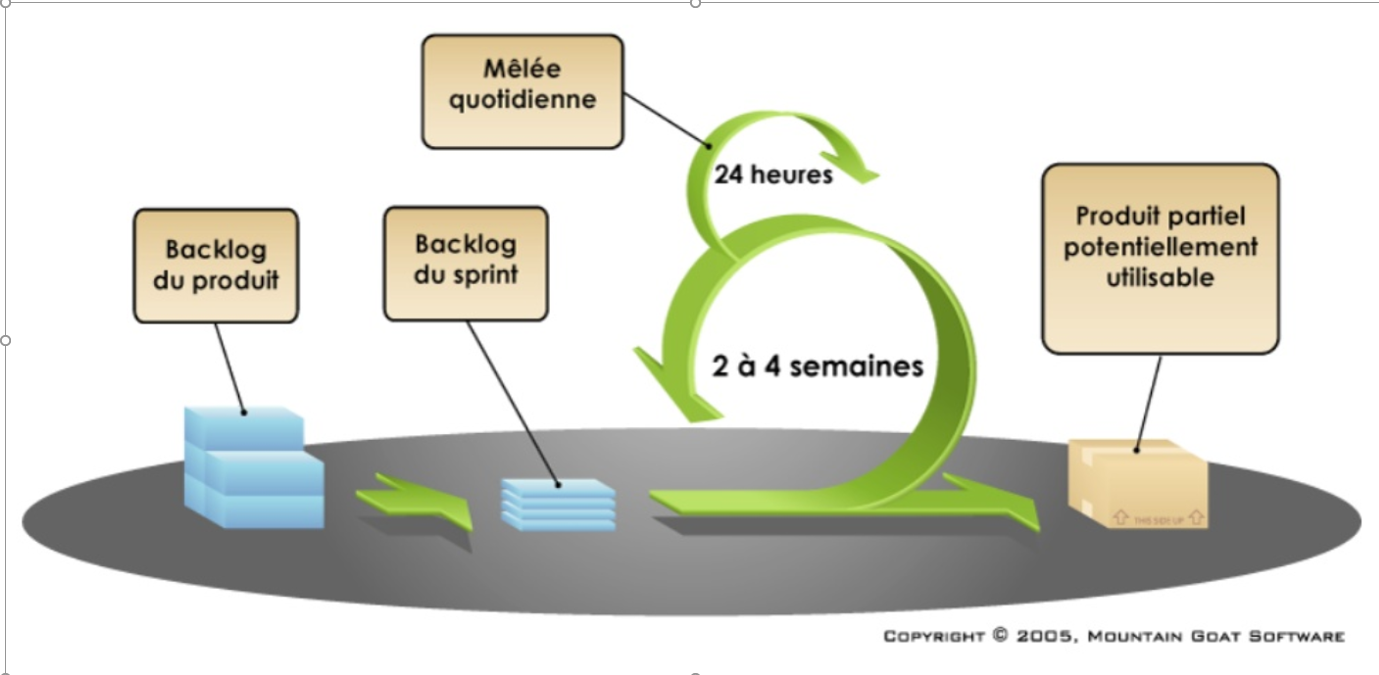
\includegraphics[width=1.1\textwidth]{scrum}
    \caption{Résumé de SCRUM}
    \label{fig:scrum}
\end{figure}

\chapter{Implementation}

\chapter*{Introduction}
\addcontentsline{toc}{chapter}{Introduction}
\markboth{Introduction}{Introduction}
\label{chap:introduction}
%\minitoc

Lorem ipsum dolor sit amet, consectetur adipiscing elit. Sed non risus. Suspendisse lectus tortor, dignissim sit amet, adipiscing nec, ultricies sed, dolor. Cras elementum ultrices diam. Maecenas ligula massa, varius a, semper congue, euismod non, mi. Proin porttitor, orci nec nonummy molestie, enim est eleifend mi, non fermentum diam nisl sit amet erat. Duis semper. Duis arcu massa, scelerisque vitae, consequat in, pretium a, enim. Pellentesque congue. Ut in risus volutpat libero pharetra tempor. Cras vestibulum bibendum augue. Praesent egestas leo in pede. Praesent blandit odio eu enim. Pellentesque sed dui ut augue blandit sodales. Vestibulum ante ipsum primis in faucibus orci luctus et ultrices posuere cubilia Curae; Aliquam nibh. Mauris ac mauris sed pede pellentesque fermentum. Maecenas adipiscing ante non diam sodales hendrerit. Ut velit mauris, egestas sed, gravida nec, ornare ut, mi. Aenean ut orci vel massa suscipit pulvinar. Nulla sollicitudin. Fusce varius, ligula non tempus aliquam, nunc turpis ullamcorper nibh, in tempus sapien eros vitae ligula. Pellentesque rhoncus nunc et augue. Integer id felis. Curabitur aliquet pellentesque diam. Integer quis metus vitae elit lobortis egestas. Lorem ipsum dolor sit amet, consectetuer adipiscing elit. Morbi vel erat non mauris convallis vehicula. Nulla et sapien. Integer tortor tellus, aliquam faucibus, convallis id, congue eu, quam. Mauris ullamcorper felis vitae erat. Proin feugiat, augue non elementum posuere, metus purus iaculis lectus, et tristique ligula justo vitae magna. Aliquam convallis sollicitudin purus. Praesent aliquam, enim at fermentum mollis, ligula massa adipiscing nisl, ac euismod nibh nisl eu lectus. Fusce vulputate sem at sapien. Vivamus leo. Aliquam euismod libero eu enim. Nulla nec felis sed leo placerat imperdiet. Aenean suscipit nulla in justo. Suspendisse cursus rutrum augue. Nulla tincidunt tincidunt mi. Curabitur iaculis, lorem vel rhoncus faucibus, felis magna fermentum augue, et ultricies lacus lorem varius purus. Curabitur eu amet.

Lorem ipsum dolor sit amet, consectetur adipiscing elit. Sed non risus. Suspendisse lectus tortor, dignissim sit amet, adipiscing nec, ultricies sed, dolor. Cras elementum ultrices diam. Maecenas ligula massa, varius a, semper congue, euismod non, mi. Proin porttitor, orci nec nonummy molestie, enim est eleifend mi, non fermentum diam nisl sit amet erat. Duis semper. Duis arcu massa, scelerisque vitae, consequat in, pretium a, enim. Pellentesque congue. Ut in risus volutpat libero pharetra tempor. Cras vestibulum bibendum augue. Praesent egestas leo in pede. Praesent blandit odio eu enim. Pellentesque sed dui ut augue blandit sodales. Vestibulum ante ipsum primis in faucibus orci luctus et ultrices posuere cubilia Curae; Aliquam nibh. Mauris ac mauris sed pede pellentesque fermentum. Maecenas adipiscing ante non diam sodales hendrerit. Ut velit mauris, egestas sed, gravida nec, ornare ut, mi. Aenean ut orci vel massa suscipit pulvinar. Nulla sollicitudin. Fusce varius, ligula non tempus aliquam, nunc turpis ullamcorper nibh, in tempus sapien eros vitae ligula. Pellentesque rhoncus nunc et augue. Integer id felis. Curabitur aliquet pellentesque diam. Integer quis metus vitae elit lobortis egestas. Lorem ipsum dolor sit amet, consectetuer adipiscing elit. Morbi vel erat non mauris convallis vehicula. Nulla et sapien. Integer tortor tellus, aliquam faucibus, convallis id, congue eu, quam. Mauris ullamcorper felis vitae erat. Proin feugiat, augue non elementum posuere, metus purus iaculis lectus, et tristique ligula justo vitae magna. Aliquam convallis sollicitudin purus. Praesent aliquam, enim at fermentum mollis, ligula massa adipiscing nisl, ac euismod nibh nisl eu lectus. Fusce vulputate sem at sapien. Vivamus leo. Aliquam euismod libero eu enim. Nulla nec felis sed leo placerat imperdiet. Aenean suscipit nulla in justo. Suspendisse cursus rutrum augue. Nulla tincidunt tincidunt mi. Curabitur iaculis, lorem vel rhoncus faucibus, felis magna fermentum augue, et ultricies lacus lorem varius purus. Curabitur eu amet.

%%% Local Variables: 
%%% mode: latex
%%% TeX-master: "isae-report-template"
%%% End: 

\chapter{Premier chapitre}
\label{chap:premierchapitre}

\section{Une section}
Lorem ipsum dolor sit amet, consectetur adipiscing elit \cite{Roque2012,Roque2012b,Roque2012c,Roque2012d}. Sed non risus. Suspendisse lectus tortor, dignissim sit amet, adipiscing nec, ultricies sed, dolor. Cras elementum ultrices diam. Maecenas ligula massa, varius a, semper congue, euismod non, mi. Proin porttitor, orci nec nonummy molestie, enim est eleifend mi, non fermentum diam nisl sit amet erat. Duis semper. Duis arcu massa, scelerisque vitae, consequat in, pretium a, enim. Pellentesque congue. Ut in risus volutpat libero pharetra tempor. Cras vestibulum bibendum augue. Praesent egestas leo in pede. Praesent blandit odio eu enim. Pellentesque sed dui ut augue blandit sodales. Vestibulum ante ipsum primis in faucibus orci luctus et ultrices posuere cubilia Curae; Aliquam nibh. Mauris ac mauris sed pede pellentesque fermentum. Maecenas adipiscing ante non diam sodales hendrerit. Ut velit mauris, egestas sed, gravida nec, ornare ut, mi. Aenean ut orci vel massa suscipit pulvinar. Nulla sollicitudin. Fusce varius, ligula non tempus aliquam, nunc turpis ullamcorper nibh, in tempus sapien eros vitae ligula. Pellentesque rhoncus nunc et augue. Integer id felis. Curabitur aliquet pellentesque diam. Integer quis metus vitae elit lobortis egestas. Lorem ipsum dolor sit amet, consectetuer adipiscing elit. Morbi vel erat non mauris convallis vehicula. Nulla et sapien. Integer tortor tellus, aliquam faucibus, convallis id, congue eu, quam. Mauris ullamcorper felis vitae erat. Proin feugiat, augue non elementum posuere, metus purus iaculis lectus, et tristique ligula justo vitae magna. Aliquam convallis sollicitudin purus. Praesent aliquam, enim at fermentum mollis, ligula massa adipiscing nisl, ac euismod nibh nisl eu lectus. Fusce vulputate sem at sapien. Vivamus leo. Aliquam euismod libero eu enim. Nulla nec felis sed leo placerat imperdiet. Aenean suscipit nulla in justo. Suspendisse cursus rutrum augue. Nulla tincidunt tincidunt mi. Curabitur iaculis, lorem vel rhoncus faucibus, felis magna fermentum augue, et ultricies lacus lorem varius purus. Curabitur eu amet (fig. \ref{fig:une-image}). Deux citations \cite{Arapoglou2011,Roque2013c}.

\begin{figure}[htp]
  \centering
  \tikzstyle{block} = [draw, fill=blue!20, rectangle, minimum height=3em, minimum width=6em, text width=6em,text centered]
\begin{tikzpicture}[auto, node distance=3.5cm,>=latex']
\shorthandoff{:} % Evite le bug de compilation avec tikz
    % Longueurs et espacement
    \def\longabove{0.2cm}
    \def\espacement{4cm}

    % Définition des blocs
    \node [block, node distance=\espacement] (codeur) {Codeur};
    \node [block, right of=codeur, node distance=\espacement] (cbs) {CBS};
    \node [block, right of=cbs, node distance=\espacement] (modulateur) {Modulateur};
 
    % Définition des liens
    \draw [<-] (codeur) -- ++(-2,0) node[left] {$\{b_n\}$};
    \draw [->] (codeur) -- node[above=\longabove] {$\{d_n\}$} (cbs);
    \draw [->] (cbs) -- node[above=\longabove] {$\{c_k\}$} (modulateur);
    \draw [->] (modulateur) -- ++(2,0) node[right] {$s(t)$};
\end{tikzpicture}

  \caption{Exemple de diagramme TikZ.}
  \label{fig:une-image}
\end{figure}

\section{Une autre section}
Lorem ipsum dolor sit amet, consectetur adipiscing elit. Sed non risus. Suspendisse lectus tortor, dignissim sit amet, adipiscing nec, ultricies sed, dolor. Cras elementum ultrices diam. Maecenas ligula massa, varius a, semper congue, euismod non, mi. Proin porttitor, orci nec nonummy molestie, enim est eleifend mi, non fermentum diam nisl sit amet erat. Duis semper. Duis arcu massa, scelerisque vitae, consequat in, pretium a, enim. Pellentesque congue. Ut in risus volutpat libero pharetra tempor. Cras vestibulum bibendum augue. Praesent egestas leo in pede. Praesent blandit odio eu enim. Pellentesque sed dui ut augue blandit sodales. Vestibulum ante ipsum primis in faucibus orci luctus et ultrices posuere cubilia Curae; Aliquam nibh. Mauris ac mauris sed pede pellentesque fermentum. Maecenas adipiscing ante non diam sodales hendrerit. Ut velit mauris, egestas sed, gravida nec, ornare ut, mi. Aenean ut orci vel massa suscipit pulvinar. Nulla sollicitudin. Fusce varius, ligula non tempus aliquam, nunc turpis ullamcorper nibh, in tempus sapien eros vitae ligula. Pellentesque rhoncus nunc et augue. Integer id felis. Curabitur aliquet pellentesque diam. Integer quis metus vitae elit lobortis egestas. Lorem ipsum dolor sit amet, consectetuer adipiscing elit. Morbi vel erat non mauris convallis vehicula. Nulla et sapien. Integer tortor tellus, aliquam faucibus, convallis id, congue eu, quam. Mauris ullamcorper felis vitae erat. Proin feugiat, augue non elementum posuere, metus purus iaculis lectus, et tristique ligula justo vitae magna. Aliquam convallis sollicitudin purus. Praesent aliquam, enim at fermentum mollis, ligula massa adipiscing nisl, ac euismod nibh nisl eu lectus. Fusce vulputate sem at sapien. Vivamus leo. Aliquam euismod libero eu enim. Nulla nec felis sed leo placerat imperdiet. Aenean suscipit nulla in justo. Suspendisse cursus rutrum augue. Nulla tincidunt tincidunt mi. Curabitur iaculis, lorem vel rhoncus faucibus, felis magna fermentum augue, et ultricies lacus lorem varius purus. Curabitur eu amet (tab. \ref{tab:un-tableau}).

\begin{table}[ht]
  \begin{center}
    \begin{tabular}{|c|c|c|c|c|}
      \hline
      & $h(t,\tau)$ & $S_{\OP{H}}^{(\alpha)} (f,\tau)$ & $L_{\OP{H}}^{(\alpha)} (\nu,t)$ & $H^{(\alpha)}(f,\nu)$ \\
      \hline
      LTI & $q(\tau)$ & $q(\tau) \delta(f)$ & $Q(\nu)$ & $Q(\nu) \delta(\nu-f)$ \\
      \hline
      LFI & $m(t) \delta(\tau)$ & $M(f) \delta(\tau)$ & $m(t)$ & $M(f)$\\
      \hline
      identité & $\delta(t)$ & $\delta(f)\delta(\tau)$ & $1$ & $\delta(\nu-f)$\\
      \hline
    \end{tabular}
    \caption{Exemple de tableau.}
    \label{tab:un-tableau}
  \end{center}
\end{table}

Lorem ipsum dolor sit amet, consectetur adipiscing elit. Sed non risus. Suspendisse lectus tortor, dignissim sit amet, adipiscing nec, ultricies sed, dolor. Cras elementum ultrices diam. Maecenas ligula massa, varius a, semper congue, euismod non, mi. Proin porttitor, orci nec nonummy molestie, enim est eleifend mi, non fermentum diam nisl sit amet erat. Duis semper. Duis arcu massa, scelerisque vitae, consequat in, pretium a, enim. Pellentesque congue. Ut in risus volutpat libero pharetra tempor. Cras vestibulum bibendum augue. Praesent egestas leo in pede. Praesent blandit odio eu enim. Pellentesque sed dui ut augue blandit sodales. Vestibulum ante ipsum primis in faucibus orci luctus et ultrices posuere cubilia Curae; Aliquam nibh. Mauris ac mauris sed pede pellentesque fermentum. Maecenas adipiscing ante non diam sodales hendrerit. Ut velit mauris, egestas sed, gravida nec, ornare ut, mi. Aenean ut orci vel massa suscipit pulvinar. Nulla sollicitudin. Fusce varius, ligula non tempus aliquam, nunc turpis ullamcorper nibh, in tempus sapien eros vitae ligula. Pellentesque rhoncus nunc et augue. Integer id felis. Curabitur aliquet pellentesque diam. Integer quis metus vitae elit lobortis egestas. Lorem ipsum dolor sit amet, consectetuer adipiscing elit. Morbi vel erat non mauris convallis vehicula. Nulla et sapien. Integer tortor tellus, aliquam faucibus, convallis id, congue eu, quam. Mauris ullamcorper felis vitae erat. Proin feugiat, augue non elementum posuere, metus purus iaculis lectus, et tristique ligula justo vitae magna. Aliquam convallis sollicitudin purus. Praesent aliquam, enim at fermentum mollis, ligula massa adipiscing nisl, ac euismod nibh nisl eu lectus. Fusce vulputate sem at sapien. Vivamus leo. Aliquam euismod libero eu enim. Nulla nec felis sed leo placerat imperdiet. Aenean suscipit nulla in justo. Suspendisse cursus rutrum augue. Nulla tincidunt tincidunt mi. Curabitur iaculis, lorem vel rhoncus faucibus, felis magna fermentum augue, et ultricies lacus lorem varius purus. Curabitur eu amet (fig. \ref{fig:une-autre-image}).

\begin{figure}[htp]
  \centering
  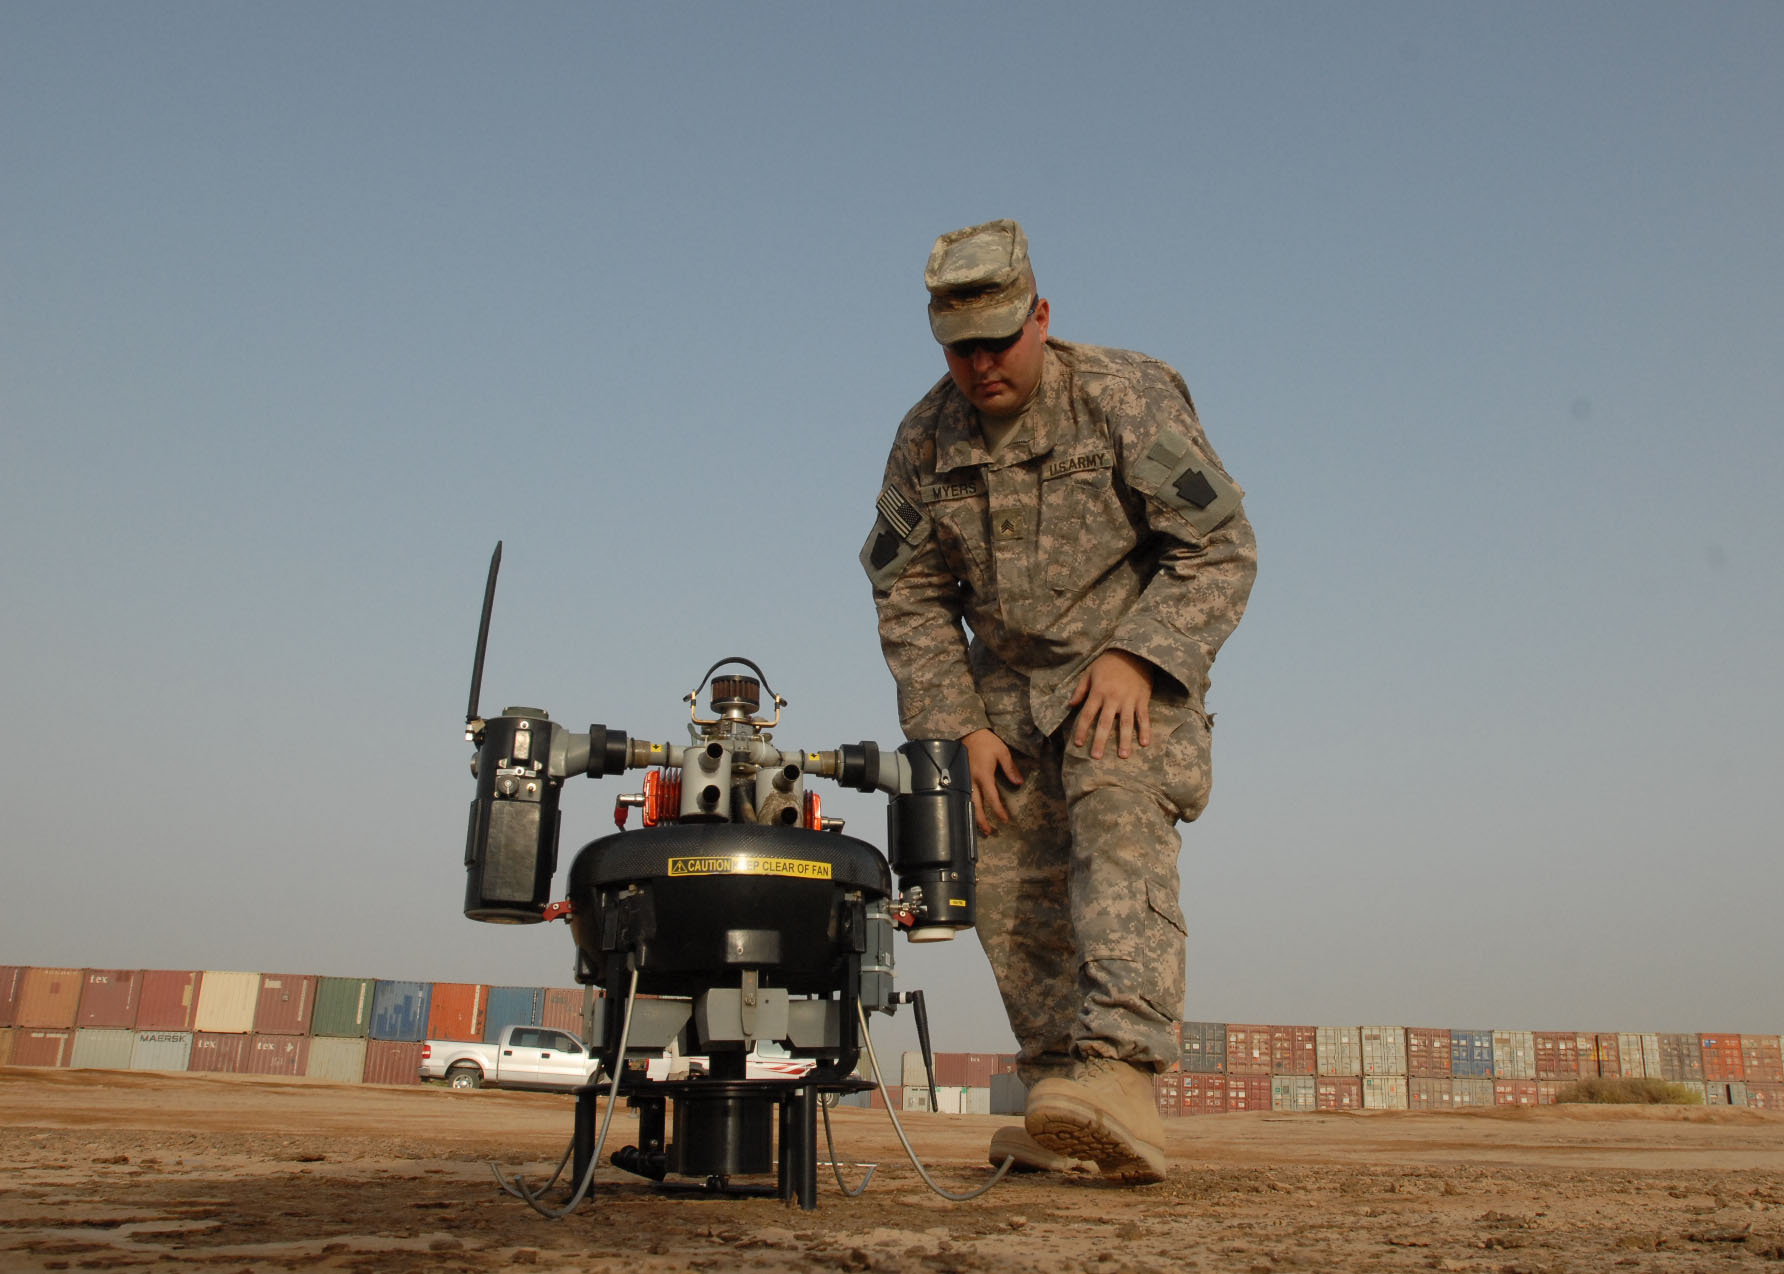
\includegraphics[width=4cm]{images/bitmap_image}
  \caption{Exemple d'image au format JPG.}
  \label{fig:une-autre-image}
\end{figure}


%%% Local Variables: 
%%% mode: latex
%%% TeX-master: "isae-report-template"
%%% End: 
\chapter{Un chapitre}
\label{sec:unchapitre}

Lorem ipsum dolor sit amet, consectetur adipiscing elit. Sed non risus. Suspendisse lectus tortor, dignissim sit amet, adipiscing nec, ultricies sed, dolor. Cras elementum ultrices diam. Maecenas ligula massa, varius a, semper congue, euismod non, mi. Proin porttitor, orci nec nonummy molestie, enim est eleifend mi, non fermentum diam nisl sit amet erat. Duis semper. Duis arcu massa, scelerisque vitae,  convallis sollicitudin purus. Praesent aliquam, enim at fermentum mollis, ligula massa adipiscing nisl, ac euismod nibh nisl eu lectus. Fusce vulputate sem at sapien. Vivamus leo. Aliquam euismod libero eu enim. Nulla nec felis sed leo placerat imperdiet. Aenean suscipit nulla in justo. Suspendisse cursus rutrum augue. Nulla tincidunt tincidunt mi. Curabitur iaculis, lorem vel rhoncus faucibus, felis magna fermentum augue, et ultricies lacus lorem varius purus. Curabitur eu amet. Encore une citation \cite{Cadambe2008}.

\begin{figure}[htp!]
  \centering
  \setlength\figureheight{7cm}
  \setlength\figurewidth{9cm}
  % This file was created by matlab2tikz v0.2.2.
% Copyright (c) 2008--2012, Nico Schlömer <nico.schloemer@gmail.com>
% All rights reserved.
% 
% 
% 

% defining custom colors
\definecolor{mycolor1}{rgb}{0,0.75,0.75}

\begin{tikzpicture}

\begin{axis}[%
view={0}{90},
width=\figurewidth,
height=\figureheight,
scale only axis,
xmin=2, xmax=4.5,
xlabel={$\eta$},
xmajorgrids,
ymin=0.5, ymax=1,
ylabel={$d_{\text{min}}^2$},
ymajorgrids,
legend cell align=left,
legend style={align=left}]
\addplot [
color=black,
dashed,
mark=asterisk,
mark options={solid}
]
coordinates{
 (2,1)(2.1,1)(2.2,1)(2.3,1)(2.4,1)(2.5,1)(2.6,0.937749781479547)(2.7,0.890900393128398)(2.8,0.864988513955105)(2.9,0.827013168393703)(3,0.811347612650328)(3.1,0.792559278041243)(3.2,0.765840563467819)(3.3,0.749680961469385)(3.4,0.741947149227874)(3.5,0.740609493518419)(3.6,0.732128087463441)(3.7,0.717775843626632)(3.8,0.699687461812158)(3.9,0.685018622769455)(4,0.673439611642851)(4.1,0.664624248264608)(4.2,0.658255928882634)(4.3,0.641702335270489)(4.4,0.608326504614558)(4.5,0.580489221369454) 
};
\addlegendentry{$\alpha\text{ =  0\%}$};

\addplot [
color=black,
dashed,
mark=x,
mark options={solid}
]
coordinates{
 (2,1)(2.1,1)(2.2,1)(2.3,1)(2.4,0.958561324724996)(2.5,0.900812804739278)(2.6,0.859608621629443)(2.7,0.828484932127753)(2.8,0.812298837741994)(2.9,0.778916291864501)(3,0.758500630955482)(3.1,0.748375165853317)(3.2,0.745960208532468)(3.3,0.738441167434538)(3.4,0.715506361296671)(3.5,0.696927131434508)(3.6,0.682276848692725)(3.7,0.671128156410174)(3.8,0.663062783265717)(3.9,0.657680299791254)(4,0.621142740976429)(4.1,0.589786339121755)(4.2,0.564530571776849)(4.3,0.54483432747474)(4.4,0.53008799514765)(4.5,0.519641830384595) 
};
\addlegendentry{$\alpha\text{ = 10\%}$};

\addplot [
color=black,
dashed,
mark=triangle,
mark options={solid}
]
coordinates{
 (2,1)(2.1,1)(2.2,1)(2.3,0.966145915091813)(2.4,0.907589260275562)(2.5,0.862273165052718)(2.6,0.833762738286283)(2.7,0.797262289343802)(2.8,0.774689700869446)(2.9,0.763077871790574)(3,0.759584455148894)(3.1,0.735410358863577)(3.2,0.713220246811223)(3.3,0.695713299974315)(3.4,0.682371019886023)(3.5,0.672682085917092)(3.6,0.6661550402729)(3.7,0.644666127799479)(3.8,0.610083129739041)(3.9,0.582172698611821)(4,0.560333265725228)(4.1,0.543883933286703)(4.2,0.532098369213191)(4.3,0.524242326405)(4.4,0.519608701974017)(4.5,0.517545187250875) 
};
\addlegendentry{$\alpha\text{ = 20\%}$};

\addplot [
color=black,
dashed,
mark=triangle,
mark options={solid,,rotate=180}
]
coordinates{
 (2,1)(2.1,1)(2.2,0.995488894312993)(2.3,0.930050749246739)(2.4,0.882604857341179)(2.5,0.840148695151764)(2.6,0.807621264874927)(2.7,0.787889977099099)(2.8,0.777972678915356)(2.9,0.750463202108443)(3,0.726620292578349)(3.1,0.707917379352703)(3.2,0.693763185722015)(3.3,0.683575144048861)(3.4,0.676795290182409)(3.5,0.663350261880571)(3.6,0.627666127013326)(3.7,0.598755039468926)(3.8,0.575986310488554)(3.9,0.558651995817327)(4,0.546003746104731)(4.1,0.537291509323841)(4.2,0.531798375059385)(4.3,0.528867181690889)(4.4,0.527917002741411)(4.5,0.528450017604181) 
};
\addlegendentry{$\alpha\text{ = 30\%}$};

\addplot [
color=black,
dashed,
mark=o,
mark options={solid}
]
coordinates{
 (2,1)(2.1,1)(2.2,1)(2.3,1)(2.4,1)(2.5,0.995096871086856)(2.6,0.937749790013923)(2.7,0.890900391028178)(2.8,0.864988509535523)(2.9,0.827013167946275)(3,0.811347609462027)(3.1,0.79255927917077)(3.2,0.765840564829299)(3.3,0.749680963181722)(3.4,0.741947149533667)(3.5,0.740609492450166)(3.6,0.732128080624777)(3.7,0.71777584554089)(3.8,0.699687463368726)(3.9,0.681193180471954)(4,0.640212533267028)(4.1,0.617585040920557)(4.2,0.608519007405809)(4.3,0.608298095410932)(4.4,0.608326494076335)(4.5,0.580489212682311) 
};
\addlegendentry{Mazo};

\end{axis}
\end{tikzpicture}%
  \caption{Exemple de courbe TikZ.}
  \label{fig:courbe-tikz}
\end{figure}

\section{Analyse aux limites}
Lorem ipsum dolor sit amet, consectetur adipiscing elit. Sed non risus. Suspendisse lectus tortor, dignissim sit amet, adipiscing nec, ultricies sed, dolor. Cras elementum ultrices diam. Maecenas ligula massa, varius a, semper congue, euismod non, mi. Proin porttitor, orci nec nonummy molestie, enim est eleifend mi, non fermentum diam nisl sit amet erat. Duis semper. Duis arcu massa, scelerisque vitae, consequat in, pretium a, enim. Pellentesque congue. Ut in risus volutpat libero pharetra tempor. Cras vestibulum bibendum augue. Praesent egestas leo in pede. Praesent blandit odio eu enim. Pellentesque sed dui ut augue blandit sodales. Vestibulum ante ipsum primis in faucibus orci luctus et ultrices posuere cubilia Curae; Aliquam nibh. Mauris ac mauris sed pede pellentesque fermentum. Maecenas adipiscing ante non diam sodales hendrerit. Ut velit mauris, egestas sed, gravida nec, ornare ut, mi. Aenean ut orci vel massa suscipit pulvinar. Nulla sollicitudin. Fusce varius, ligula non tempus aliquam, nunc turpis ullamcorper nibh, in tempus sapien eros vitae ligula. Pellentesque rhoncus nunc et augue. Integer id felis. Curabitur aliquet pellentesque diam. Integer quis metus vitae elit lobortis egestas. Lorem ipsum dolor sit amet, consectetuer adipiscing elit. Morbi vel erat non mauris convallis vehicula. Nulla et sapien. Integer tortor tellus, aliquam faucibus, convallis id, congue eu, quam. Mauris ullamcorper felis vitae erat. Proin feugiat, augue non elementum posuere, metus purus iaculis lectus, et tristique ligula justo vitae magna. Aliquam convallis sollicitudin purus. Praesent aliquam, enim at fermentum mollis, ligula massa adipiscing nisl, ac euismod nibh nisl eu lectus. Fusce vulputate sem at sapien. Vivamus leo. Aliquam euismod libero eu enim. Nulla nec felis sed leo placerat imperdiet. Aenean suscipit nulla in justo. Suspendisse cursus rutrum augue. Nulla tincidunt tincidunt mi. Curabitur iaculis, lorem vel rhoncus faucibus, felis magna fermentum augue, et ultricies lacus lorem varius purus. Curabitur eu amet.

\subsection{Quelques détails sur cette méthode}
Lorem ipsum dolor sit amet, consectetuer adipiscing elit. Morbi vel erat non mauris convallis vehicula. Nulla et sapien. Integer tortor tellus, aliquam faucibus, convallis id, congue eu, quam. Mauris ullamcorper felis vitae erat. Proin feugiat, augue non elementum posuere, metus purus iaculis lectus, et tristique ligula justo vitae magna. Aliquam convallis sollicitudin purus. Praesent aliquam, enim at fermentum mollis, ligula massa adipiscing nisl, ac euismod nibh nisl eu lectus. Fusce vulputate sem at sapien. Vivamus leo. Aliquam euismod libero eu enim. Nulla nec felis sed leo placerat imperdiet. Aenean suscipit nulla in justo. Suspendisse cursus rutrum augue. Nulla tincidunt tincidunt mi. Curabitur iaculis, lorem vel rhoncus faucibus, felis magna fermentum augue, et ultricies lacus lorem varius purus. Curabitur eu amet.

\subsection{On n'est jamais très fort pour ce calcul}
Lorem ipsum dolor sit amet, consectetuer adipiscing elit. Morbi vel erat non mauris convallis vehicula. Nulla et sapien. Integer tortor tellus, aliquam faucibus, convallis id, congue eu, quam. Mauris ullamcorper felis vitae erat. Proin feugiat, augue non elementum posuere, metus purus iaculis lectus, et tristique ligula justo vitae magna. Aliquam convallis sollicitudin purus. Praesent aliquam, enim at fermentum mollis, ligula massa adipiscing nisl, ac euismod nibh nisl eu lectus. Fusce vulputate sem at sapien. Vivamus leo. Aliquam euismod libero eu enim. Nulla nec felis sed leo placerat imperdiet. Aenean suscipit nulla in justo. Suspendisse cursus rutrum augue. Nulla tincidunt tincidunt mi. Curabitur iaculis, lorem vel rhoncus faucibus, felis magna fermentum augue, et ultricies lacus lorem varius purus. Curabitur eu amet.

\begin{align}
H_{m,n,p,q} &= \DPR{\rproto_{p,q}}{\OP{H} \tproto_{m,n}}\\
&= \iint\limits_{\SET{R}^2} S_{\OP{H}}(f,\tau) \DPR{\rproto_{p,q}}{\OP{U}_{f,\tau} \tproto_{m,n}} \ud f \ud \tau.
\end{align}

\section{Vérification par simulation numérique}
Lorem ipsum dolor sit amet, consectetur adipiscing elit. Sed non risus. Suspendisse lectus tortor, dignissim sit amet, adipiscing nec, ultricies sed, dolor. Cras elementum ultrices diam. Maecenas ligula massa, varius a, semper congue, euismod non, mi. Proin porttitor, orci nec nonummy molestie, enim est eleifend mi, non fermentum diam nisl sit amet erat. Duis semper. Duis arcu massa, scelerisque vitae, consequat in, pretium a, enim. Pellentesque congue. Ut in risus volutpat libero pharetra tempor. Cras vestibulum bibendum augue. Praesent egestas leo in pede. Praesent blandit odio eu enim. Pellentesque sed dui ut augue blandit sodales. Vestibulum ante ipsum primis in faucibus orci luctus et ultrices posuere cubilia Curae; Aliquam nibh. Mauris ac mauris sed pede pellentesque fermentum. Maecenas adipiscing ante non diam sodales hendrerit. Ut velit mauris, egestas sed, gravida nec, ornare ut, mi. Aenean ut orci vel massa suscipit pulvinar. Nulla sollicitudin. Fusce varius, ligula non tempus aliquam, nunc turpis ullamcorper nibh, in tempus sapien eros vitae ligula. Pellentesque rhoncus nunc et augue. Integer id felis. Curabitur aliquet pellentesque diam. Integer quis metus vitae elit lobortis egestas. Lorem ipsum dolor sit amet, consectetuer adipiscing elit. Morbi vel erat non mauris convallis vehicula. Nulla et sapien. Integer tortor tellus, aliquam faucibus, convallis id, congue eu, quam. Mauris ullamcorper felis vitae erat. Proin feugiat, augue non elementum posuere, metus purus iaculis lectus, et tristique ligula justo vitae magna. Aliquam convallis sollicitudin purus. Praesent aliquam, enim at fermentum mollis, ligula massa adipiscing nisl, ac euismod nibh nisl eu lectus. Fusce vulputate sem at sapien. Vivamus leo. Aliquam euismod libero eu enim. Nulla nec felis sed leo placerat imperdiet. Aenean suscipit nulla in justo. Suspendisse cursus rutrum augue. Nulla tincidunt tincidunt mi. Curabitur iaculis, lorem vel rhoncus faucibus, felis magna fermentum augue, et ultricies lacus lorem varius purus. Curabitur eu amet.

%%% Local Variables: 
%%% mode: latex
%%% TeX-master: "isae-report-template"
%%% End: 
\chapter*{Conclusion et perspectives}
\addcontentsline{toc}{chapter}{Conclusion}
\markboth{Conclusion}{Conclusion}
\label{sec:conclusion}

    Lorem ipsum dolor sit amet, consectetur adipiscing elit. Sed non risus. Suspendisse lectus tortor, dignissim sit amet, adipiscing nec, ultricies sed, dolor. Cras elementum ultrices diam. Maecenas ligula massa, varius a, semper congue, euismod non, mi. Proin porttitor, orci nec nonummy molestie, enim est eleifend mi, non fermentum diam nisl sit amet erat. Duis semper. Duis arcu massa, scelerisque vitae, consequat in, pretium a, enim. Pellentesque congue. Ut in risus volutpat libero pharetra tempor. Cras vestibulum bibendum augue. Praesent egestas leo in pede. Praesent blandit odio eu enim. Pellentesque sed dui ut augue blandit sodales. Vestibulum ante ipsum primis in faucibus orci luctus et ultrices posuere cubilia Curae; Aliquam nibh. Mauris ac mauris sed pede pellentesque fermentum. Maecenas adipiscing ante non diam sodales hendrerit. Ut velit mauris, egestas sed, gravida nec, ornare ut, mi. Aenean ut orci vel massa suscipit pulvinar. Nulla sollicitudin. Fusce varius, ligula non tempus aliquam, nunc turpis ullamcorper nibh, in tempus sapien eros vitae ligula. Pellentesque rhoncus nunc et augue. Integer id felis. Curabitur aliquet pellentesque diam. Integer quis metus vitae elit lobortis egestas. Lorem ipsum dolor sit amet, consectetuer adipiscing elit. Morbi vel erat non mauris convallis vehicula. Nulla et sapien. Integer tortor tellus, aliquam faucibus, convallis id, congue eu, quam. Mauris ullamcorper felis vitae erat. Proin feugiat, augue non elementum posuere, metus purus iaculis lectus, et tristique ligula justo vitae magna. Aliquam convallis sollicitudin purus. Praesent aliquam, enim at fermentum mollis, ligula massa adipiscing nisl, ac euismod nibh nisl eu lectus. Fusce vulputate sem at sapien. Vivamus leo. Aliquam euismod libero eu enim. Nulla nec felis sed leo placerat imperdiet. Aenean suscipit nulla in justo. Suspendisse cursus rutrum augue. Nulla tincidunt tincidunt mi. Curabitur iaculis, lorem vel rhoncus faucibus, felis magna fermentum augue, et ultricies lacus lorem varius purus. Curabitur eu amet.

%%% Local Variables: 
%%% mode: latex
%%% TeX-master: "isae-report-template"
%%% End: 



\appendix

\bibliographystyle{authoryear-fr}
\bibliography{references}

\clearpage

%%%%%%%%%%%%%%%%
%%% Abstract %%%
%%%%%%%%%%%%%%%%

\thispagestyle{empty}

\vspace*{\fill}
\noindent\rule[2pt]{\textwidth}{0.5pt}\\
{\textbf{Résumé ---}}
Lorem ipsum dolor sit amet, consectetur adipiscing elit. Sed non risus. Suspendisse lectus tortor, dignissim sit amet, adipiscing nec, ultricies sed, dolor. Cras elementum ultrices diam. Maecenas ligula massa, varius a, semper congue, euismod non, mi. Proin porttitor, orci nec nonummy molestie, enim est eleifend mi, non fermentum diam nisl sit amet erat. Duis semper. Duis arcu massa, scelerisque vitae, consequat in, pretium a, enim. Pellentesque congue. Ut in risus volutpat libero pharetra tempor. Cras vestibulum bibendum augue. Praesent egestas leo in pede. Praesent blandit odio eu enim. Pellentesque sed dui ut augue blandit sodales. Vestibulum ante ipsum primis in faucibus orci luctus et ultrices posuere cubilia Curae; Aliquam nibh. Mauris ac mauris sed pede pellentesque fermentum. Maecenas adipiscing ante non diam sodales hendrerit. Ut velit mauris, egestas sed, gravida nec, ornare ut, mi. Aenean ut orci vel massa suscipit pulvinar. Nulla sollicitudin. Fusce varius, ligula non tempus aliquam, nunc turpis ullamcorper nibh, in tempus sapien eros vitae ligula. Pellentesque rhoncus nunc et augue. Integer id felis.

{\textbf{Mots clés :}}
Lorem ipsum dolor sit amet, consectetur adipiscing elit. Sed non risus. Suspendisse lectus tortor.
\\
\noindent\rule[2pt]{\textwidth}{0.5pt}
\begin{center}
  ISAE\\
  10, avenue Édouard Belin\\
  BP 54032\\
  31055 Toulouse CEDEX 4
\end{center}
\vspace*{\fill}

\end{document}